\documentclass[tikz,border=6pt]{standalone}
\usepackage{amsmath,amssymb}
\usetikzlibrary{arrows.meta,calc,shadows.blur}
\colorlet{cR}{red!72!black}
\colorlet{cB}{blue!62!black}
\begin{document}
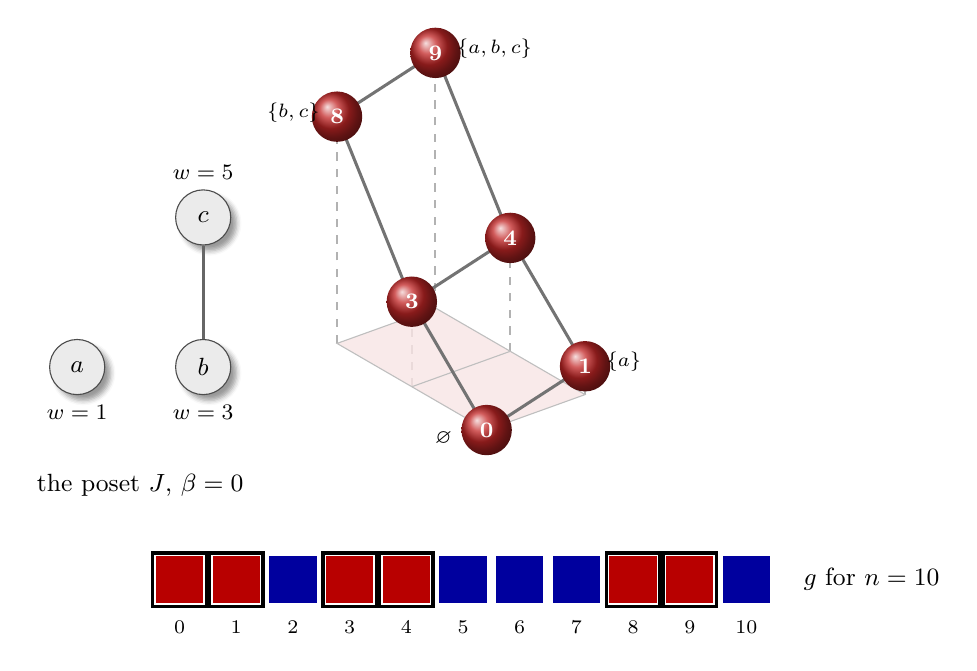
\begin{tikzpicture}[
  el/.style={circle,draw=black!70,fill=black!8,minimum size=7mm,inner sep=0pt,font=\small,blur shadow},
  node3/.style={circle,ball color=cR!85!white,minimum size=6.4mm,inner sep=0pt,text=white,font=\footnotesize\bfseries},
  edge3/.style={line width=1.1pt,black!55},
  back3/.style={line width=0.7pt,black!30,dashed}]
% --- the weighted poset J
\begin{scope}[shift={(-5.2,0.8)}]
  \node[el] (a) at (0,0) {$a$};
  \node[el] (b) at (1.6,0) {$b$};
  \node[el] (c) at (1.6,1.9) {$c$};
  \draw[line width=1pt,black!60] (b) -- (c);
  \node[font=\footnotesize,anchor=north] at (a.south) {$w=1$};
  \node[font=\footnotesize,anchor=north] at (b.south) {$w=3$};
  \node[font=\footnotesize,anchor=south] at (c.north) {$w=5$};
  \node[font=\small] at (0.8,-1.5) {the poset $J$, $\beta=0$};
\end{scope}
% --- its lattice of down-sets, drawn in space with height = size
\begin{scope}[x={(1.25cm,0.45cm)},y={(-0.95cm,0.55cm)},z={(0cm,0.36cm)}]
  % floor grid (coordinates: first = membership of a, second = level in chain b<c)
  \foreach \i in {0,1} \foreach \j in {0,1,2}
     \draw[back3] (\i,\j,0) -- (\i,\j,{ \i*1 + (\j>0)*3 + (\j>1)*5 });
  \fill[cR!10,opacity=0.8] (0,0,0) -- (1,0,0) -- (1,2,0) -- (0,2,0) -- cycle;
  \draw[black!25] (0,0,0) -- (1,0,0) -- (1,2,0) -- (0,2,0) -- cycle (0,1,0)--(1,1,0);
  \coordinate (p00) at (0,0,0);  \coordinate (p10) at (1,0,1);
  \coordinate (p01) at (0,1,3);  \coordinate (p11) at (1,1,4);
  \coordinate (p02) at (0,2,8);  \coordinate (p12) at (1,2,9);
  \draw[edge3] (p00)--(p10) (p01)--(p11) (p02)--(p12) (p00)--(p01)--(p02) (p10)--(p11)--(p12);
  \node[node3] at (p00) {0}; \node[node3] at (p10) {1};
  \node[node3] at (p01) {3}; \node[node3] at (p11) {4};
  \node[node3] at (p02) {8}; \node[node3] at (p12) {9};
  \node[font=\scriptsize,anchor=west] at ($(p10)+(0.12,0,0)$) {$\{a\}$};
  \node[font=\scriptsize,anchor=east] at ($(p00)+(-0.25,0,0)$) {$\varnothing$};
  \node[font=\scriptsize,anchor=west] at ($(p12)+(0.12,0,0)$) {$\{a,b,c\}$};
  \node[font=\scriptsize,anchor=east] at ($(p02)+(0,0.1,0)$) {$\{b,c\}$};
\end{scope}
% --- the colouring word for n = 10
\begin{scope}[shift={(-4.2,-2.2)}]
  \foreach \c [count=\i from 0] in {R,R,B,R,R,B,B,B,R,R,B}{
    \if R\c\def\col{cR}\else\def\col{cB}\fi
    \fill[\col] (0.72*\i,0) rectangle ++(0.6,0.6);
    \node[font=\scriptsize] at (0.72*\i+0.3,-0.3) {\i};
  }
  \foreach \i in {0,1,3,4,8,9}{\draw[line width=1.2pt,black] (0.72*\i-0.04,-0.04) rectangle ++(0.68,0.68);}
  \node[font=\small,anchor=west] at (8.1,0.3) {$g$ for $n=10$};
\end{scope}
\end{tikzpicture}
\end{document}
